\subsection{拟紧集；紧集；相对紧集}

定义 2. 拓扑空间 X 的子集 A 称为拟紧集（相应地，紧集），如果子空间 A 是拟紧的（相应地，紧的）。

拓扑空间 X 的子集 A 是拟紧集，当且仅当每个由 X 的开集组成的 A 的覆盖都包含 A 的一个有限覆盖；这由公理 (C'\,') 得出。在豪斯多夫空间中，拟紧集与紧集这两个概念相同，因为每个子空间都是豪斯多夫的。

例. 1) 在拓扑空间 X 中，每个有限子集都是拟紧的；空集与每个单点集都是紧的。2) 在拓扑空间 X 中，设 \((x_{n})_{n\in \mathbb{N}}\) 是收敛于一点 \(a\) 的一个无穷点列；则由诸点 \(x_{n}\)（\(n\in \mathbb{N}\)）与 \(a\) 组成的集合 A 是拟紧的。因为若 \((\mathrm{U}_{\iota})\) 是由 X 的开集组成的 A 的一个覆盖，则 \(a\in \mathrm{U}_{\iota}\) 对某个指标 \(\iota\) 成立。\(\mathrm{U}_{\iota}\) 是 \(a\) 的邻域，因此只有有限多个指标 \(n_k\) 使 \(x_{nk}\notin \mathrm{U}_{\iota}\)。对每个指标 \(k\)，设 \(\iota_{k}\) 是使 \(x_{nk}\in \mathrm{U}_{\iota_{k}}\) 的一个指标；则 \(\mathrm{U}_{\iota}\) 与诸 \(\mathrm{U}_{\iota_{k}}\) 构成 A 的一个有限开覆盖。

命题 3. 拟紧（相应地，紧）空间的每个闭子集都是拟紧（相应地，紧）的。

只要注意到：若 A 在 X 中是闭的，则在 A 中闭的每个集合在 X 中也是闭的，这便是公理 (C'') 的直接推论。

命题 4. 豪斯多夫空间的每个紧子集都是闭的。

设 A 是豪斯多夫空间 X 的一个紧子集，并设 x 是 \(\overline{A}\) 的任一点；我们要证明 \(x \in A\)。由假设，x 的每个邻域都与 A 相交，因此 x 在 X 中的邻域滤子 B 在 A 上诱导一个滤子 \(B_{A}\)；A 是紧的，故 \(B_{A}\) 有一个聚点 \(y \in A\)。既然滤子 B 比 \(B_{A}\)（视为 X 上的一个滤子基）在 X 上生成的滤子更粗，y 也是 B 的聚点；于是 y = x，因为 B 在 X 中收敛于 x，且 X 是豪斯多夫的（§ 8，第 1 目，命题 1）。

推论. 在紧空间 X 中，子集 A 是紧的，当且仅当它在 X 中是闭的。

命题 5. 拓扑空间中拟紧子集的一个有限族的并是拟紧的。

只需证明：若 A 与 B 是拓扑空间 X 的两个拟紧子集，则 \(A \cup B\) 是拟紧的。设 R 是 \(A \cup B\) 的一个覆盖；则 R 既是 A 的覆盖又是 B 的覆盖；于是 R 包含 A 的一个有限覆盖 \(R_{1}\) 与 B 的一个有限覆盖 \(R_{2}\)；从而 \(R_{1} \cup R_{2}\) 是 \(A \cup B\) 的一个包含于 R 中的有限覆盖。

定义 3. 拓扑空间 X 的子集 A 称为 X 中相对拟紧（相应地，相对紧）的，如果 A 包含于 X 的一个拟紧（相应地，紧）子集之中。

为简便起见，当关于 X 没有歧义时，我们也说 A 是“相对拟紧集”（相应地，“相对紧集”）。在豪斯多夫空间中，相对拟紧集与相对紧集这两个概念相同。

命题 6. 若 X 是豪斯多夫空间，则 X 的子集 A 是相对紧的，当且仅当 \(\overline{A}\) 是紧的。

若 A 是相对紧的，则由命题 4 及其推论，\(\overline{A}\) 是紧的；反向的蕴含是显而易见的。

命题 7. 若 A 是拓扑空间 X 的一个相对拟紧子集，则 A 上的每个滤子基在 X 中都有一个聚点。

因为若 \(\mathbf{A} \subset \mathbf{K}\)，其中 \(\mathbf{K}\) 是 \(\mathbf{X}\) 的一个拟紧子集，则 \(\mathbf{A}\) 上的每个滤子基在 \(\mathbf{K}\) 中都有一个聚点。

这个命题的逆命题在对 X 不加限制时并不成立（习题 22）。

\pandocbounded{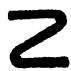
\includegraphics[keepaspectratio]{images/part001_f875b0ae.jpg}}

注. 在非豪斯多夫空间中，紧集未必是闭的，其闭包也未必是拟紧的（习题 5）；两个紧集的交未必是拟紧的（习题 5）；两个紧集的并未必是紧的（习题 5）。

